% A literate Haskell file
------------------------------------------------------------------------------
\section{Specifying the DOM's Foundations \note{4pp}}
\label{sec:specifying}

\subsection{[Motivating Specification]}
% REMEMBER: [terms: complies with standard, compatible with]

\begin{lstlisting}[style=meta]
- an implementation
  - should comply with the standard
  - should safely support less than standard
  - pragmatically support some common extant data malformations so as to be compatible with extant data
  - should carefully support more than the standard
  - should not "inf. loop"
    - lots of opportunities - failure to notice digitally signed PDFs that have been tampered!
    - where failure leads to "parser differential" without user warning (e.g. excessive trailer /Size)
    - PDF requires "backwards parsing" which is unnatural for many programming languages
      - elaborate?
\end{lstlisting}

\begin{lstlisting}[style=meta]
- Lack of formality in standard. Thus, implementations:
  - are more effort
  - over implement, under implement, wrongly implement
  - backwards and forwards compatibility
  - "backwards parsing"
  - some requirements will not be checked by PDF readers ("writer only" file requirements) 
  - patch existing vs implement from scratch
- No definition of acceptable, reasonable error recovery
- Less than ideal design that reflects 27 years of an evolving standard
- Pre-DOM processing
  - is where many parsing errors & recovery occur
  - is non-trivial
  - involves multiple interdependent features and subtle dialects
  - involves multiple redundant features
    - schizophrenic if these features aren't mutually consistent
\end{lstlisting}

\subsection{The Major PDF File Components}

\begin{figure}[t]
    \centering
    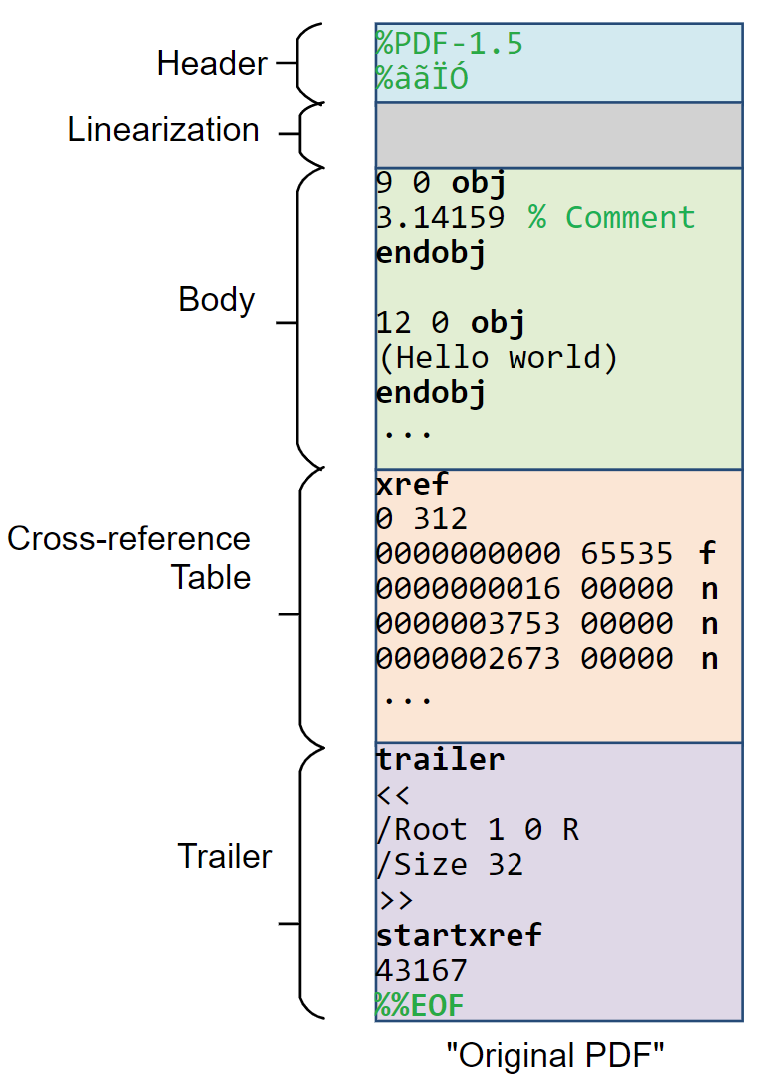
\includegraphics[width=0.35\linewidth]{figures/pdf-structure.png}
    \caption{PDF File Structure.}
    \label{fig:pdf-structure}
\end{figure}

The overall structure of a PDF is shown in \cref{fig:pdf-structure}.
\todo{short paragraph: describe overall PDF doc structure}

\todo{import the type definitions and go into a little more detail}
  
\subsection{Specifying pre-DOM components}

%%%% Hs code not in paper %%%%
\iffalse
\begin{code}
{-# LANGUAGE EmptyDataDecls, TypeOperators, LambdaCase #-}
module Spec where

import           Control.Monad
import           Data.Char
import           Data.Foldable(foldlM)
import qualified Data.Map as M
import           Data.Map(Map)

import           Types
import           Utils
import           Primitives
\end{code}
\fi

In what follows we use Haskell \cite{Haskell} as a specification language for
our specification.
%
Our goal is to bridge the gap between the lowest level parsers
(parsing integers, parsing xref entries, etc.) and the processing
that happens after the DOM is created.   Thus, the primitive parsers
are omitted from this spec as well as a few other simple functions.
See \cref{sec:appendix1} for the Haskell type signatures for
the parsing primitives and other omitted functions.
The full spec can be found online at \todo{where?}.

\begin{itemize}
\item The specification is formal and executable\footnote{
  Executable does not imply efficient, the specification is written
  primarily to be \emph{clear}.}.
  %
  This is our motivation for choosing Haskell over pseudo-code, english prose,
  and non-executable formalisms.  For the reader without a reading knowledge of
  Haskell, we understand that parts of the specification may be a little
  unclear, but our hope is that a precise, formal specification may prove to be
  more useful than pseudo-code or the like!
  
\item The specification is purely functional: no global variables are hidden,
  the data-dependencies in the spec fully represent all the data-dependencies.
  
\item The specification hides no difficulties: one could implement a PDF parser
  by writing the omitted functions, but the spec stands complete, as is!
\end{itemize}

\todo{MT: turn old bullet points/comments below into prose!}

\begin{code}
pPDFDom :: P DOM
pPDFDom =
    do
    -- find '%PDF-x.y' at start of file, skipping up to 1K bytes:
    (version,headerFileOffset) <- findPDFHeader
    -- search backwards from EOF for 'startxref', gives up after 1000 bytes:
    (startxrefOff,xrefOff) <- findStartxrefThenParseToEOF
\end{code}

\todo{introduce P and Haskell 'do'? (elsewhere?)}
  
\begin{code}  
    let jmp n = setInputAt (headerFileOffset+n)
    jmp xrefOff
\end{code}

\todo{there are places where we need to add calls to \lstcd{jmp}.}
  
\begin{code}  
    (xrefRaw, xrefEndOff) <- pXrefRaw :: P (XRefRaw,Offset)
    validate $
      verifyXrefRaw xrefRaw
      -- - this ensures no duplicate objectIds
      -- - we could, but don't need to (yet)
      --   - parse xref entries
      --   - validate xref entries (without parsing the object)
    jmp xrefEndOff
       -- Because pXrefSubSections doesn't need to parse contents of
       -- the subsections.
\end{code}

At this point (without parsing sections)
 - we know the list of objects
 - we can find xref entry for each object
 - we know the end of xref table
but the above is predicated on
 - enforcing full standard compliance with 20 byte (only) xref entries.
   - currently 19,21 byte xref entries are considered NCBUR!
if we were to allow 19-21 byte xref entries:
  - we would be nothing essential would 
  - nothing essential would 


\begin{code}
    trailerDict <- pSimpleWhiteSpace >> keyword "trailer" >> pDictionary
    validate $
      do
      cs <- readTo startxrefOff
      return (all isSpace cs)
    trailerDict' <- dictToTrailerDict trailerDict

    let mPrev = trailerDict_getPrev trailerDict' :: Maybe Offset
        etc = trailerDict_Extras trailerDict'    :: Dict
          -- etc is a list of unknown key-value pairs
          -- we could be even lazier to allow
          --  - Xref and DOM analysis even when errors in dictionary

\end{code}

\begin{code}
    updates' <- pAllUpdates mPrev :: P [(XRefRaw, TrailerDict)]
       -- we've followed the 'Prev's and for each
       --   - pXrefRaw     -- processed xref subsections (at raw level)
       --   - pTrailerDict -- similar to above, but
       --                     only reads/validates Prev key
\end{code}

at this point
 - we have
   - parsed/validated minimally
   - rejected *some* invalid PDFs
   - no PDF 'values' parsed except trailer dictionaries
 - we can (without further 'parsing' or reading of input)
   - output trailer dictionaries
   - output high level info wrt incremental updates
 - we've detected
   - overlapping ObjIds in an xref table (and ...?)
 - we have NOT
   - parsed anything inessential to creating DOM
   - parsed the contents of xref entries

\begin{code}  
    let updates = (xrefRaw,trailerDict) : updates'
    dom <- makeDOMFromUpdates jmp updates

    -- N.B.: only when we have parsed everything, do we
    -- actually know the PDF version, because the version
    -- may be embedded in the DOM:
    version' <- updateVersionFromCatalogDict dom version
    if version' > (2,0) then
      warn "PDF file has version greater than 2.0"
    else
      -- version' <= (2,0)
      when (not (null etc)) $
        warn "trailer dictionary has unknown keys (per PDF 2.0)"
    return dom
\end{code}

The \lstcd{pDOM} function definition is now finished, but most of
the work has been put in the \lstcd{makeDOMFromUpdates} function,
where we create the DOM from the list of incremental updates:

\begin{code}
makeDOMFromUpdates :: (Offset -> P ()) -> [(XRefRaw, TrailerDict)] -> P DOM
makeDOMFromUpdates jmp updates =
    do
    -- combine all the updates to get a single map to offsets:
    xrefs <- combineAllXrefTables updates
             :: P (Map ObjId (Offset :+: Type2Ref))

    -- at this point
    --  - we know ALL the object ids in PDF

    -- parse all uncompressed objects (but leave streams undecoded):
    domPass1 <- mapM
                  (mMapLeft (\o-> do {jmp o; pTopLevelDef_UnDecStm}))
                  xrefs
                :: P (Map ObjId (TopLevelDef_UnDecStm :+: Type2Ref))
\end{code}

\todo{don't call the results of pass 1 'domPass'.}

we are only NOW able to
  - verify/read toplevel stream data
    - b/c now indirect /Length and ... is defined in domPass1
    - decode ObjStm streams (if 1.5+)
    
\begin{code}
    -- decode streams into ByteStrings, also pre-processes ObjStm streams
    domPass2 <- mapM
                  (mMapLeft (extractStreamData domPass1))
                  domPass1
                :: P (Map ObjId (TopLevelDef :+: Type2Ref))
\end{code}

at this point
 - can compute body cavities
 - ObjStm's have been pre-processed
   - but objects inside them not parsed

\begin{code}
    domFinal <- mapM
                 (return `either` derefType2Ref domPass2)
                  domPass2
                :: P (Map ObjId TopLevelDef)
    return domFinal
\end{code}

at this point
 - every object referenced via xref has been parsed
 - However,
   - extraneous object defs in body are never parsed
   - unreferenced objects (per xref) in ObjStm's are never parsed
 - we positively know the PDF version (only now)
   - catalog dictionary might have been in an ObjStm
   - Q. is this intentional? this precludes lots of checks.

\subsection{Details of Streams and Type 2 References}

\begin{code}
-- | extractStreamData - since we now know all Lengths:
--   - 1st, with the file offset, read into a bytestring
--   - 2nd, if an ObjStm, decodes/validates the stream
--     - NOTE: this processing done just once, not each time
--       that we "index" into the ObjStm.
extractStreamData ::
     Map ObjId (TopLevelDef' Offset :+: a)
  -> TopLevelDef' Offset
  -> P (TopLevelDef' ByteString)
extractStreamData _dom' (TLD_ObjStm _)    = error "unexpeced ObjStm"
extractStreamData _dom' (TLD_Value v)     = return $ TLD_Value v
extractStreamData dom' (TLD_Stream d off) =
  do
  len  <- getKeyOfType "Length" T_Int d  -- indirect OR direct
  len' <- derefValue dom' len            -- now an integer direct
  decodingParameters
       <- extractDecodingParameters d
  bs   <- decodeStream len' decodingParameters off
  return $ TLD_Stream d bs

derefType2Ref ::
     Map ObjId (TopLevelDef :+: Type2Ref)
  -> Type2Ref
  -> P TopLevelDef
derefType2Ref dom' (Type2Ref oi j) =
  do
  tld       <- derefTLD dom' (oi,0)
  ObjStm ss <- getObjStm tld      -- make sure the object is ObjStm
  s         <- case safeIndex ss j of
                 Just s  -> return s
                 Nothing -> error "bad type2 ref: index out of bounds"
  v <- parseString pValue s
       -- note that streams cannot be inside ObjStm
  return $ TLD_Value v

getObjStm :: TopLevelDef' ByteString -> P ObjStm
getObjStm (TLD_ObjStm x) = return x
getObjStm _              = error "expected ObjStm"
\end{code}
   
\subsection{Can we Avoid Multiple Phases?}

\todo{compare the above with a monolithic approach that APPEARS
  to not need multiple phases.}

\subsection{Elaborating on Updates}
   
\begin{code}
-- | combineAllXrefTables updates - 
--   - for each update
--     - parses each xref subsection into a list of xref entries
--   - merges all the xref tables into a single mapping
--     - when no errors/inconsistencies
combineAllXrefTables
  :: [(XRefRaw, TrailerDict)] -> P (Map ObjId (Offset :+: Type2Ref))
combineAllXrefTables updates =
  do
  updates' <- mapM pUpdate updates  
  indices' <- mapM (createIndex . fst) updates' 
  index    <- foldlM mergeIndices M.empty indices'
  return index
\end{code}

NOTE
 - we've lost information:
   - which update an object is part of
   - object history
   - object definitions that are no longer reachable
 - fails on
   - malformed xref entries
   - mixture of xref table and xref streams [PW?]
 - should detect (or fail) on
   - trailer dicts that aren't consistent between updates
   - incremental updates that are "weird/nonsensical"
     - free-ing dead objects
     - unconventional use of generation numbers
         
 - IF updates are defined by xref STREAMS
   - no problem: as we can fully parse xref stream (w/ dict) as
     there is no dependence of xref STREAMS on DOM
     - NOTE: clarificaton to PDF working group regarding this.
   - we'll have Type2Ref's in addition to Offset's
      
 - NOTE 
   - when the latter, the ObjectId -> Offset must be available
       - in current or previous (or next!) xref stream
         - BTW, pervasive design issue: must partial updates be valid?



